\documentclass{article}
\usepackage{ctex}
\usepackage[a4paper, left=2.5cm, right=2.5cm, top=2.54cm, bottom=2.54cm]{geometry}
\usepackage{graphicx}
\usepackage{caption}
\usepackage{subcaption}
\usepackage{multirow}
\usepackage{multicol}
\usepackage{booktabs}
\usepackage[normalem]{ulem}
\usepackage{eqparbox}
\usepackage{listings}
\usepackage{mdframed}
\usepackage{amsmath}
\usepackage{enumerate}
\usepackage{placeins}
\usepackage{float}
\usepackage[dvipsnames]{xcolor}  % 使用 xcolor 包的 dvipsnames 选项
\usepackage[table,xcdraw]{xcolor}
\usepackage{tikz}
\usepackage{svg}
\usetikzlibrary{shapes.geometric, arrows}
% \usepackage{minted}
\useunder{\uline}{\ul}{}
\definecolor{code_bgc}{RGB}{255, 253, 253}  % 定义一个非常淡的粉色
\lstset{
    numbers=left,                   % 在左侧显示行号
    language=[x86masm]Assembler,    % 设置语言
    numberstyle=\color{Lavender},  % 设置行号的样式
    % frame=single,                   % 添加框架
    rulecolor=\color{black},        % 设置框架的颜色
    tabsize=2,                      % 设置tab的宽度
    breaklines=true,                % 自动折行
    breakatwhitespace=false,        % 在空白处折行
    escapeinside={\%*}{*)},         % 如果你想在代码中添加LaTeX代码,可以在此处设置
    keywordstyle=\color{RedViolet},      % 设置关键字的颜色
    commentstyle=\color{Salmon},   % 设置注释的颜色
    stringstyle=\color{RoyalBlue},      % 设置字符串的颜色
    basicstyle=\footnotesize,       % 设置代码的字体大小
    columns=fullflexible, 
    xleftmargin=2em,                % 设置左边距
    backgroundcolor=\color{code_bgc}, % 设置背景颜色
}


\begin{document}

\begin{table}
    \begin{tabular}{clllll}
    \multicolumn{4}{c}{\multirow{3}{*}{
\includegraphics[width=4.5cm]{assets/image.png}
    \fontsize{30}{35}\selectfont\kaishu 实验报告}}            & \quad 专业: & {\ul{\eqparbox{col4}{\quad 电子信息工程 \quad}}}     \\
    \multicolumn{4}{c}{}                                      & \quad 姓名: & {\ul {\eqparbox{col4}{\qquad 冯静怡}}}        \\
    \multicolumn{4}{c}{}                                      & \quad 学号: & {\ul {\eqparbox{col4}{\quad 3220104119}}} \\
    课程名称: & {\ul {\eqparbox{col1}{\quad 微机原理及应用实验\quad}}} & \quad 指导老师:    & {\ul {\eqparbox{col2}{胡斯登\quad}}} 
     & \quad 地点: & {\ul {\eqparbox{col4}{ 紫金港东三406}}}   \\
    实验名称: & {\ul {\eqparbox{col1}{\quad 数字计时器\quad }}}       & &
    &\quad 日期: & {\ul {\eqparbox{col4}{\today}}}      
    \end{tabular}
\end{table}

\section{实验目的}
\begin{enumerate}
    \item 学习使用单片机的各种接口
    \item 学会按键扫描和数码管扫描显示
    \item 学会使用定时器中断的状态机运行方式
\end{enumerate}

\section{实验过程}
\subsection{分析实验完成功能}
\begin{enumerate}
    \item 自定义倒计时时间;
    \item 按“开始/暂停”键实现倒计时开始,再次按“开始/暂停”键暂停倒计时;
    \item 若当前计时为00-00,按“开始/暂停”开始正计时功能,再次按“开始/暂停”,可暂停正计时功能;
    \item 按归零键,可使计时归零;
    \item 数码管显示第4~8位显示数字00-00。
\end{enumerate}
\subsection{分配硬件功能}
\begin{enumerate}
    \item 确定按键及其功能(\#XXH表示按键编号)
    \begin{itemize}
        \item \#00H 十秒位增1;\#01H 分钟个位增一;\#02H 分钟十位增一
        \item \#08H 归零;\#0BH 开始/暂停
    \end{itemize}
    \item 计时器状态,使用RAM 44H位置记录当前状态(\#XXH表示44H内存储数字)
    \begin{itemize}
        \item \#0FH 暂停
        \item \#FFH 倒计时模式;\#00H 正计时模式
        \item \#F0H 待机模式
        \item \#AAH 倒计时完成
    \end{itemize}
    实验中计时器一共可能处于以上5个状态,使用44H记录方便在代码的任何位置确认当前计时器状态
    \item 53H-57H地址位置记录当前显示的数字
    \item 22H位地址位置记录当前显示是否被清零
    \begin{itemize}
        \item 0 $\rightarrow$ 清零
        \item 1 $\rightarrow$ 有数字
    \end{itemize}
    方便确认按开始键是进行正计时/倒计时
    \item 计时器功能分配
    \begin{itemize}
        \item TIME0: 每隔10ms对键盘进行扫描;进行键盘按键的确定;但实际上为了T0的中断和T1的中断不冲突,所以设置非
        整数倍,为9548us。\\
        设置:
        $$
        T0=(65536-9548)D=(DA\ B4)H
        $$
        \item TIME1: 每隔2ms对数码管进行扫描显示。\\
        所以设置:
        $$
        T1=(65536-2000)D=(F8\ 30)H
        $$
        4AH\&4BH地址位置记录1s计数器,用于计时器的计时。
        $$
        4BH\&4AH\text=10000H-500D=(FE\ 0C)H
        $$
        45H地址位置记录暂停状态下的10s计数器,通过4AH\&4BH地址位置记录的1s计数器标志计数。
    \end{itemize}
    \item 30H地址位置记录按键按下的次数。30H=2时,开始判断按键的值(按键防抖)。当按键松开以后(30H被清零),开始执行按下按键后的对应操作。
\end{enumerate}
\subsection{代码流程}
\begin{figure}[H]
    \centering
    \includegraphics*[width=0.99\textwidth]{assets/flowchart.pdf}
\end{figure}
\newpage
\section{代码编写}
\subsection{主程序初始化}
通过下面的初始化代码,也可以分析得到各个存储单元在接下来的复杂代码中
启到的作用。
\begin{multicols}{3}
\begin{lstlisting}
    MAIN:
    ; 初始化显示的数字
    MOV R1,#53H
    LOOP_MAIN:
    MOV @R1,#00H
    INC R1
    CJNE R1,#58H,LOOP_MAIN
    MOV R1,#53H
    MOV 42H,#0F7H
    MOV 55H,#0DH
    ; 此时为零状态
    CLR 22H
    ; 八位数码管显示状态为灭灯状态
    MOV P2,#0FFH ;灯全灭
    MOV P0,#0FFH;P0口的显示值
    ; 计时器初始化
    MOV 30H,#00H    ; 按键次数初始化
    MOV TMOD,#11H   ; 设定定时器0、1工作方式
    MOV TH0,#0DAH   ; 设定定时器0初值
    MOV TL0,#0B4H
    ; 启动定时器0
    SETB EA     
    SETB ET0
    SETB TR0
    ; 设定定时器1初值,但不启动定时器1
    MOV TH1,#0F8H
    MOV TL1,#050H
    ; 设定定时器状态为待机状态
    MOV 44H,#0F0H

    MOV 45H,#00H    ; 暂停->待机状态的10s计数器
    MOV 46H,#0FFH   ; 报警状态计数器
    MOV 4AH,#0CH    ; 1s计数器,采用32位正计数方式
    MOV 4BH,#0FEH   
    MOV DPTR,#TABLE ; 查表
\end{lstlisting}
\end{multicols}
\subsection{主程序循环代码}
\begin{figure}[H]
    \begin{minipage}{0.6\textwidth}
        \hspace*{2em}主要为了在计时器结束之后能够响铃,如果计时器结束则调用响铃子程序;在执行这段代码的过程中会被定时器中断
        不断打断,但不影响主要功能。
    \end{minipage}
    \begin{minipage}{0.35\textwidth}
        \centering
        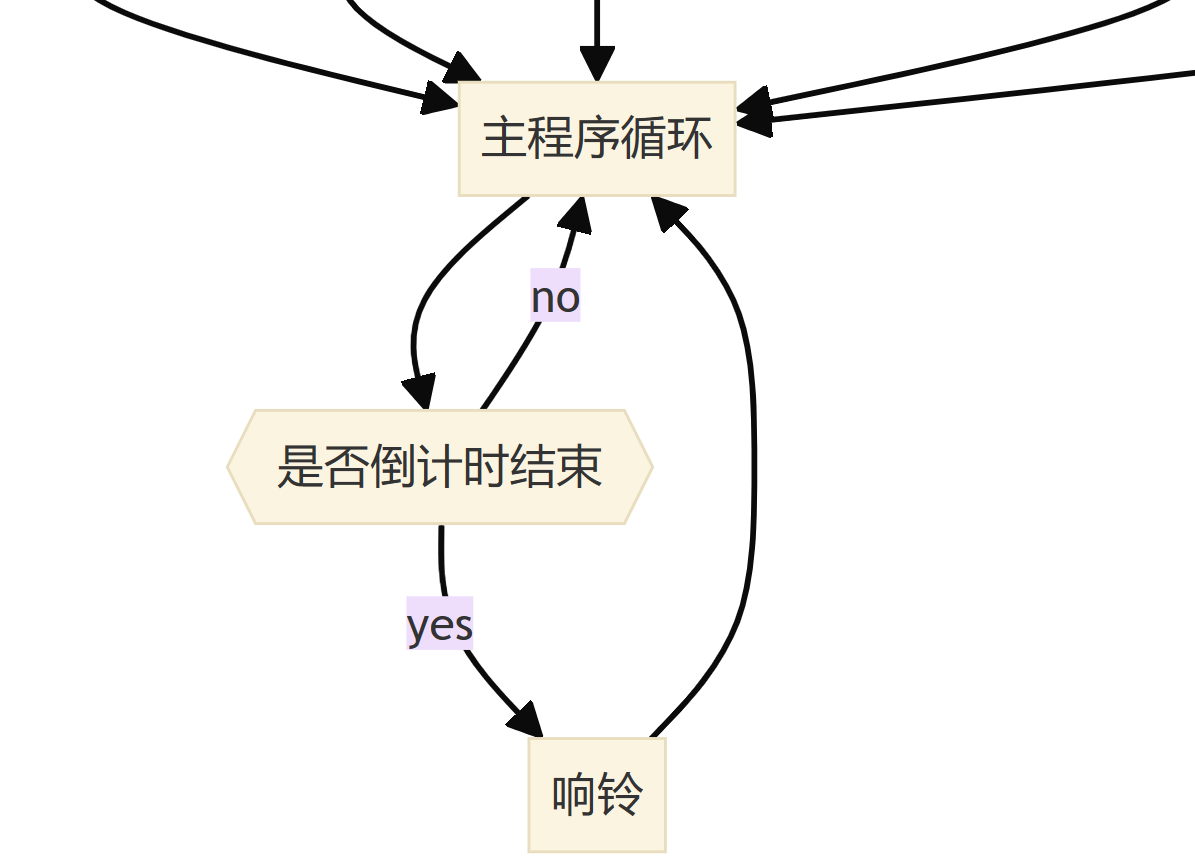
\includegraphics[width=0.8\textwidth]{assets/image-20240501180521563.png}
        \caption{主程序循环代码示意图}
    \end{minipage}
\end{figure}
\begin{multicols}{3}
    \begin{lstlisting}
LOOP_SJMP:
    MOV A,44H
    CJNE A,#0AAH,NEXT_SJMP
	    CPL	P3.4        ;取反小喇叭(p3.3)
	    LCALL	DELAY   ;调用延时
    NEXT_SJMP:
SJMP LOOP_SJMP  ;循环

DELAY:                    ;延时子程序
    MOV	R7,#00H
    LLA:
        DJNZ R7,LLA
RET
    \end{lstlisting}
\end{multicols}
\subsection{定时器T0中断子程序}
中断程序主要用于扫描按键,根据按键的情况进行相应的操作。
\begin{figure}[H]
\begin{minipage}{0.3\textwidth}
        \centering
        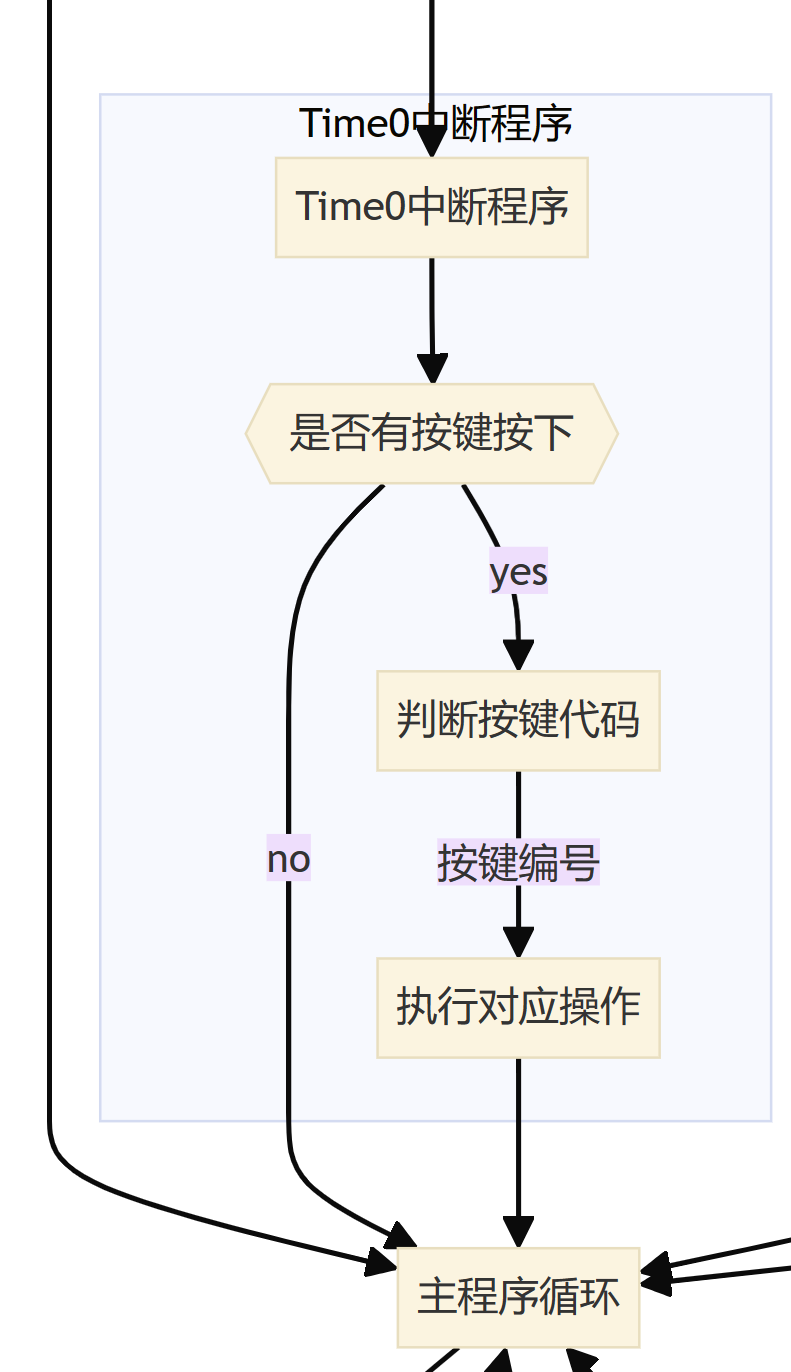
\includegraphics[width=0.99\textwidth]{assets/image-20240501181015810.png}
        \caption{TIME0运行逻辑图}
\end{minipage}
\begin{minipage}{0.667\textwidth}
\paragraph*{TIME0 中断主程序}
调用子函数KS,判断是否有按键按下;
同时记录按键按下的次数,当按键按下次数大于2次,且此时按键已经松开,跳转到OPERATE子程序。
\begin{multicols}{2}
\begin{lstlisting}
    ;定时器0中断,扫描按键
    TIME0:
        PUSH A
        PUSH PSW
        MOV TH0,#0DAH
        MOV TL0,#0B4H
        LCALL KS
        JNZ K1  ;如果有按键按下,跳转到K1
        ;如果没有按键按下,判断是什么情况下没有按下
        MOV A,30H
        JZ T0_END1   ;如果30H为0,返回中断
        CJNE A,#01H,OPERATE   ;如果30H不等于1,跳转到操作NEXT1_TIME0
        ;如果30H等于1,则将30H清零,返回中断
        MOV 30H,#00H
        LJMP T0_END1
    \end{lstlisting}
\end{multicols}
\paragraph{K1 判断按键值}
K1通过将P1口分别输出\#0F0H和\#0FH,得到具体按键。
存储为如下形式: 0001 0001B,代表第一行第一列的按键。
\begin{multicols}{2}
\begin{lstlisting}[firstnumber=16]
    K1:
        INC 30H
        MOV A,30H
        CJNE A,#02H,T0_END1  ;如果30H没两次,则返回中断
        ;30H判断按下两次,开始判断是哪一个被按下
        MOV P1,#0FH
        MOV A,P1
        CPL A
        ANL A,#0FH
        PUSH A
    
        MOV P1,#0F0H
        MOV A,P1
        CPL A
        ANL A,#0F0H
        MOV R4,A
        POP A
        ORL A,R4
\end{lstlisting}    
\end{multicols}
\end{minipage}
\end{figure}
\paragraph*{LK 按键值转换}
将形如0010 0001B的代码转化位4D的十进制数,
方便后续操作,具体代码略。
\begin{multicols}{3}
    \begin{lstlisting}[firstnumber=34]
LK:
    MOV R4,#00H
    PUSH A
LOOP:
    RRC A
    JC NEXT1
    INC R4
    CJNE R4,#04H,LOOP
    NEXT1:PUSH ACC
    MOV A,R4
    MOV B,#04H
    MUL AB
    MOV R5,A
    POP ACC

    POP ACC
    SWAP A
    MOV R4,#0H
LOOP2:
    RRC A
    JC NEXT2
    INC R4
    CJNE R4,#04H,LOOP2

    NEXT2:MOV A,R5
    ADD A,R4
    MOV 31H,A
    ; 返回中断
    \end{lstlisting}  
\end{multicols}

\paragraph*{OPERATE 按键操作}  
根据按键的值,进行相应的操作。逻辑如下图所示:
\begin{figure}[H]
    \centering
    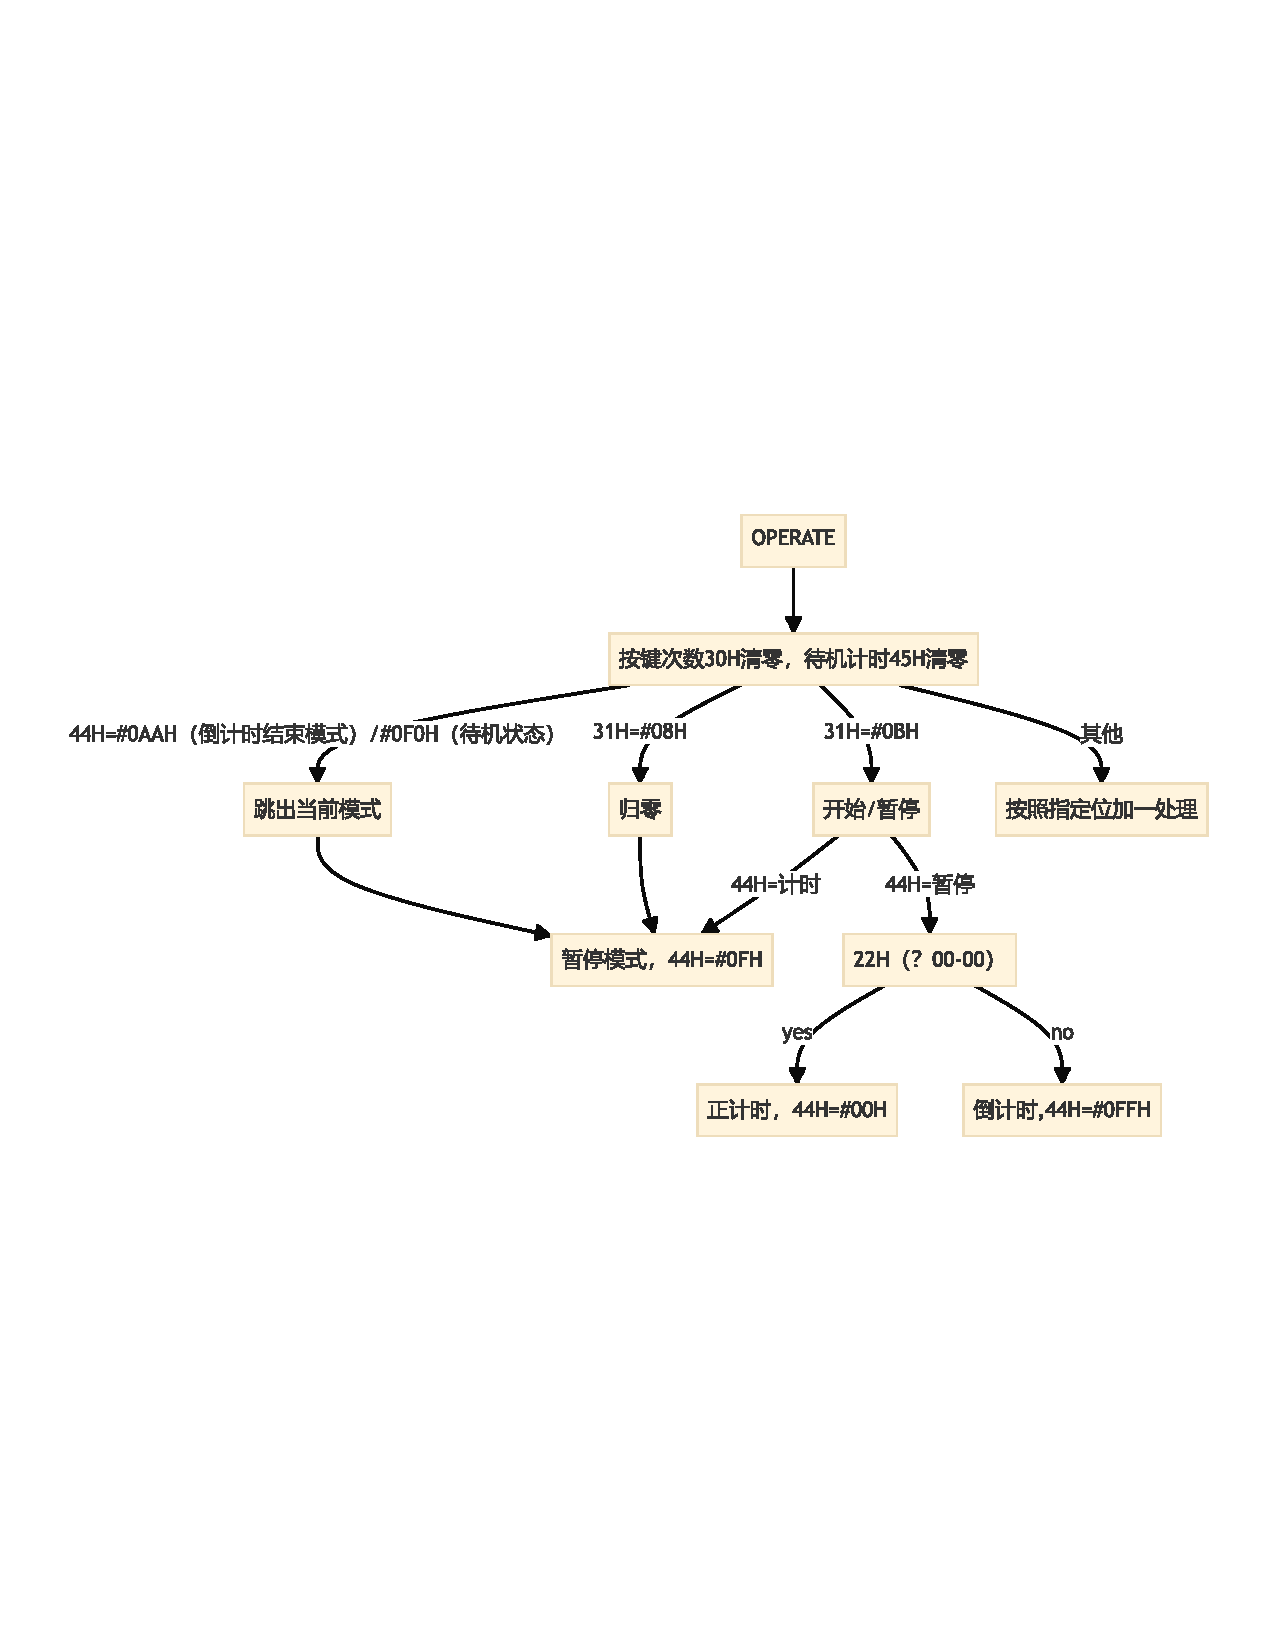
\includegraphics[width=0.8\textwidth]{assets/time0.pdf}
\end{figure}
具体代码如下:
\begin{multicols}{3}
\begin{lstlisting}[firstnumber=68]
    OPERATE:
    MOV 30H,#00H
    MOV A,44H
    MOV 45H,#00H
    CJNE A,#0AAH,NEXTXX_OPERATE
        MOV 44H,#0FH
        LJMP T0_END
    NEXTXX_OPERATE:
    CJNE A,#0F0H,NEXTX_OPERATE
    ; 息屏模式下
        MOV 44H,#0FH    ;调整为暂停模式
        SETB ET1
        SETB TR1
        MOV 42H,#0F7H ;P2口的值
        MOV R1,#53H
        LJMP T0_END
    NEXTX_OPERATE:
    MOV A, 31H
    ;判断31H的值
    ; 08H 归零
    CJNE A,#08H,OPERATE1
        CLR 22H
        MOV 44H,#0FH
        MOV R0,#53H
        LOOP_OPERATE:
        MOV @R0,#00H
        INC R0
        CJNE R0,#58H,LOOP_OPERATE
        MOV R0,#53H
        ; MOV 52H,#0DH
        MOV 55H,#0DH
        LJMP T0_END
    
    ; 0BH 开始/暂停
    OPERATE1:CJNE A,#0BH,OPERATE2
        MOV A,44H
        CJNE A,#0FH,NEXT1_OPERATE1
        ; 如果是暂停状态下
        JB 22H,NEXT2_OPERATE1
        MOV 44H,#00H
        SJMP CONTINUE_OPERATE1
        NEXT2_OPERATE1:
        MOV 44H,#0FFH
        CONTINUE_OPERATE1:
        MOV TH1,#0F8H
        MOV TL1,#030H
        LJMP T0_END
        ; 如果是计时状态下
        NEXT1_OPERATE1:
            MOV 44H,#0FH
            LJMP T0_END

    OPERATE2:
        SETB 22H
        CJNE A,#00H,OPERATE3
        MOV A,56H
        INC A
        MOV 56H,A
        CJNE A,#06H,T0_END
        MOV 56H,#00H
        SJMP JUDGEM1_OPERATE
    OPERATE3:CJNE A,#01H,OPERATE4
        JUDGEM1_OPERATE:
        MOV A,54H
        INC A
        MOV 54H,A
        CJNE A,#0AH,T0_END
        MOV 54H,#00H
        SJMP JUDGEM2_OPERATE
    OPERATE4:CJNE A,#02H,T0_END
        JUDGEM2_OPERATE:
        MOV A,53H
        INC A
        MOV 53H,A
        CJNE A,#0AH,T0_END
        MOV 53H,#00H
\end{lstlisting}
\end{multicols}

\subsection{定时器TIME1中断子程序}
\paragraph*{TIME1 中断主程序}
扫描显示数码管,一个灯亮2ms,具有四种显示状态,分别为暂停显示、正计时、倒计时、倒计时结束显示,具体逻辑如下图所示:
\begin{figure}[H]
    \begin{subfigure}{0.3\textwidth}
        \centering
        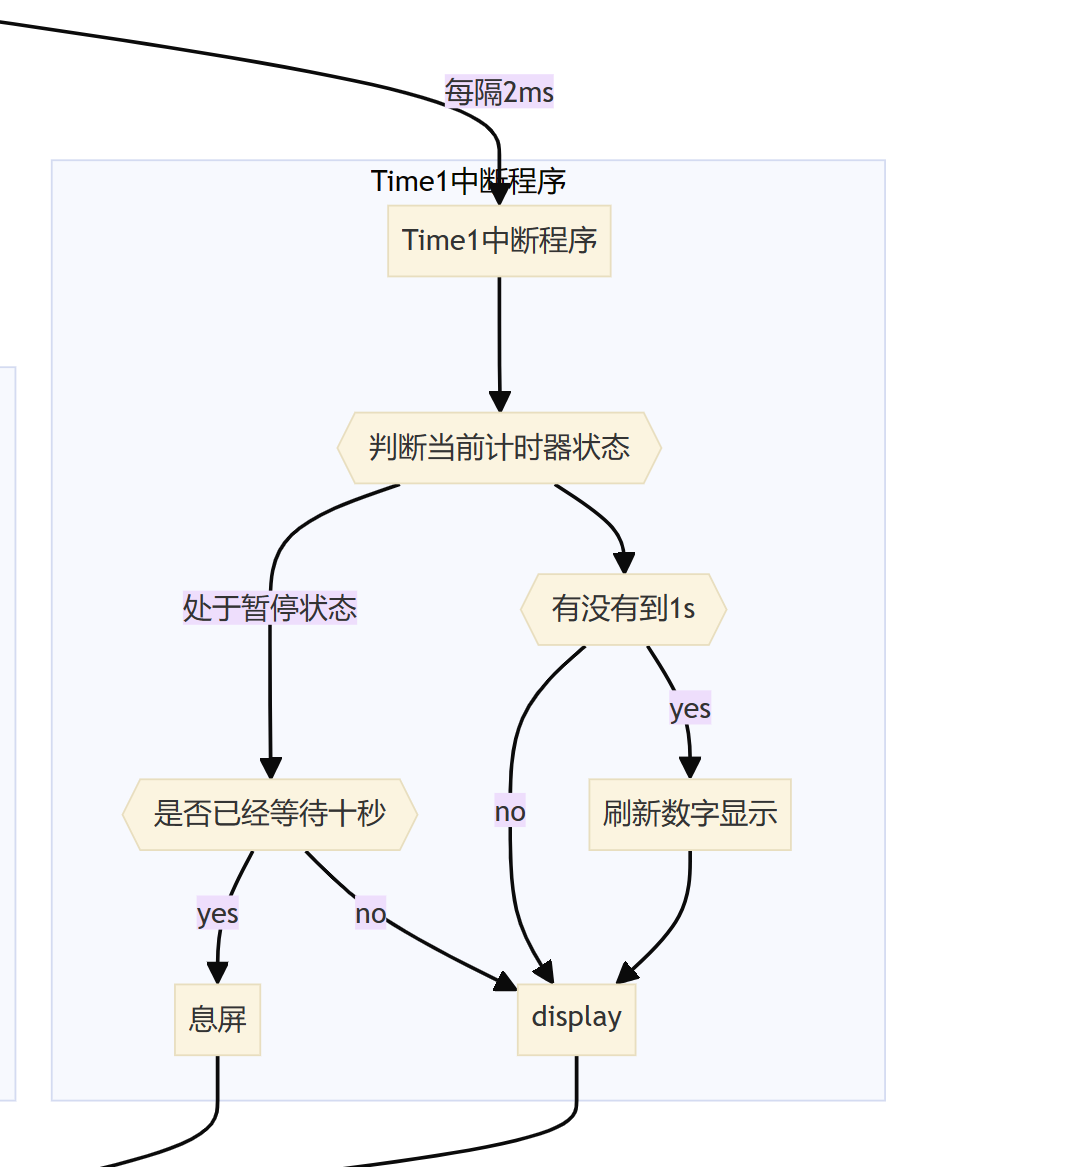
\includegraphics[width=0.99\textwidth]{assets/image-20240501210725402.png}
        \caption{TIME1运行逻辑图}
    \end{subfigure}
    \begin{subfigure}{0.69\textwidth}
        \centering
        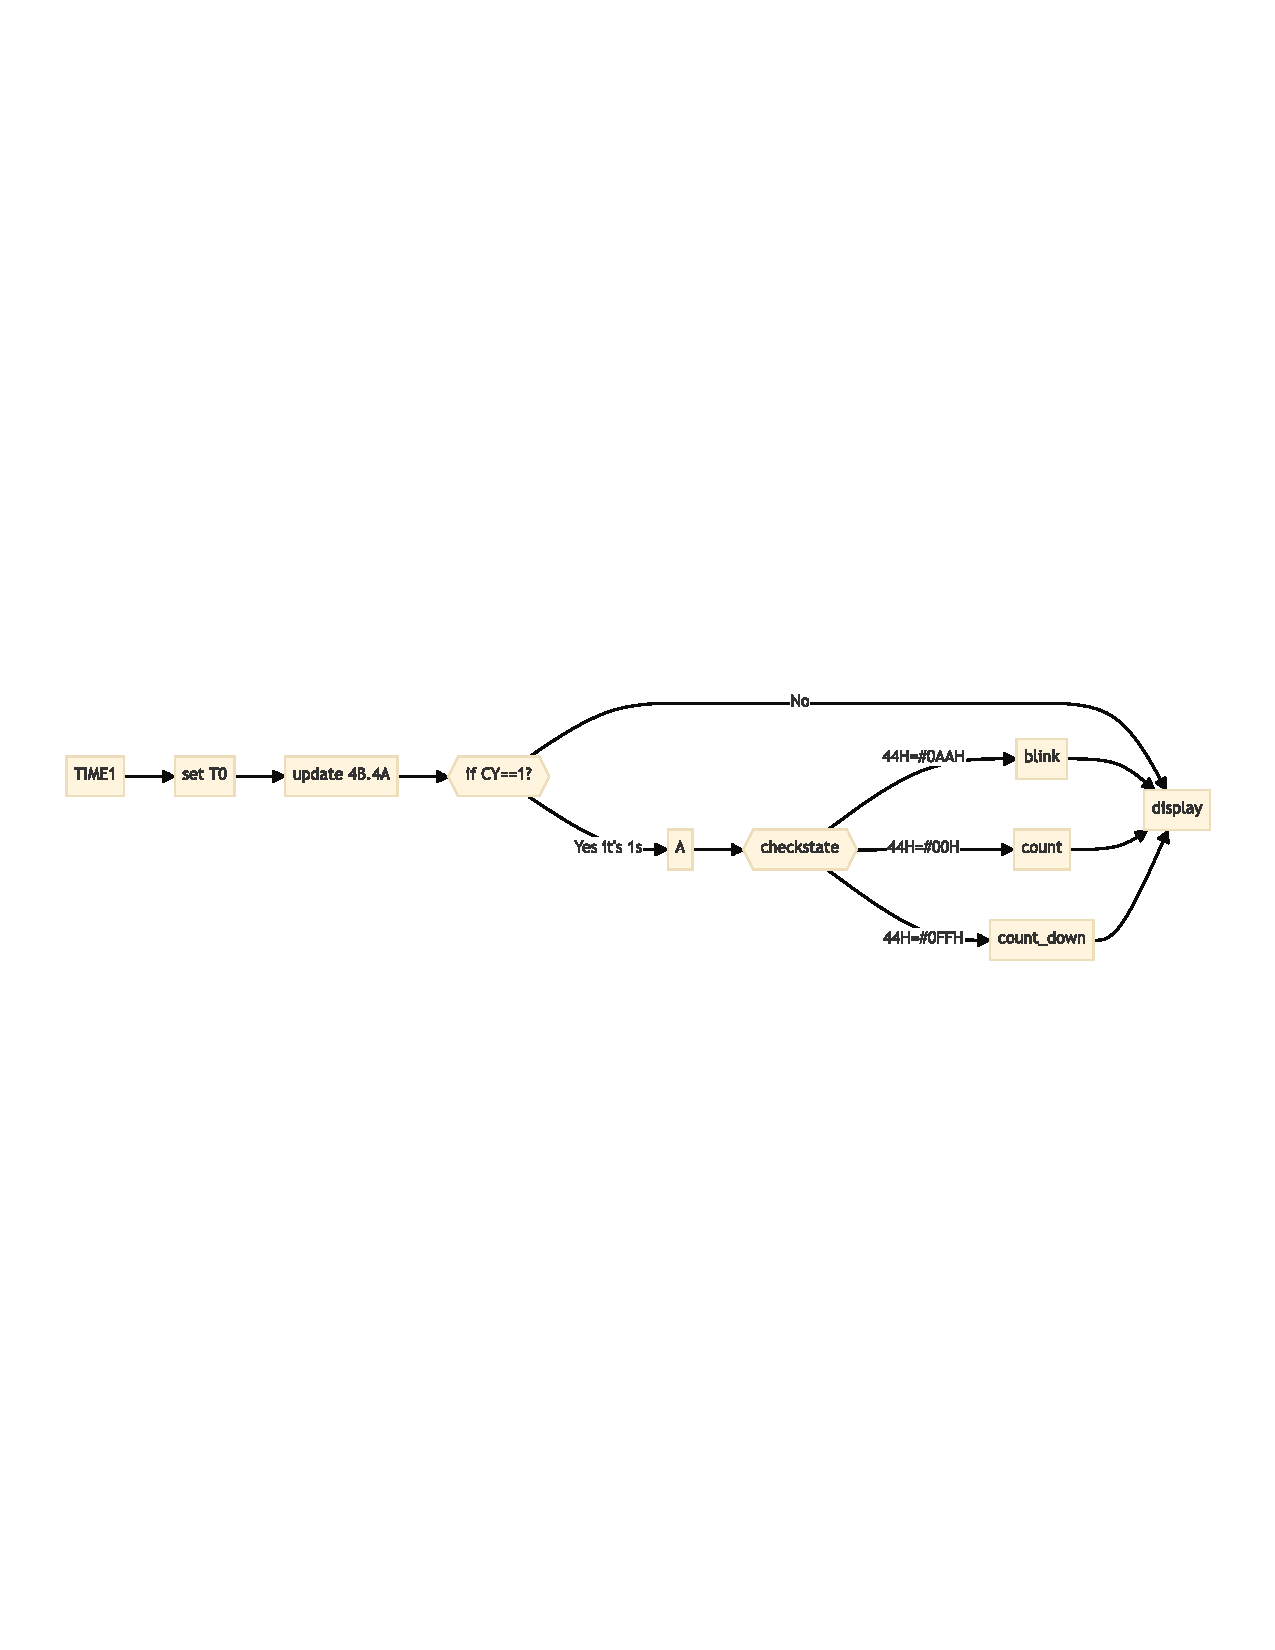
\includegraphics[width=0.99\textwidth]{assets/time1.pdf}
        \caption{TIME1具体执行方式} 
    \end{subfigure}
\end{figure}
\begin{multicols}{3}
\begin{lstlisting}
    ;扫描显示数码管
TIME1:
    PUSH A
    PUSH PSW
    ;扫描显示数码管,一个灯亮2ms
    MOV TH1,#0F8H
    MOV TL1,#030H

    MOV A,4AH
    ADD A,#01H
    MOV 4AH,A
    MOV A,4BH
    ADDC A,#00H
    MOV 4BH,A
    ;如果进位了,说明1S已经到了
    MOV A,#00H
    MOV ACC.0,C
    PUSH A
    ; 此时栈顶是标志位C
    JNC NEXT8_TIME1
    MOV 4AH,#0CH
    MOV 4BH,#0FEH

    NEXT8_TIME1:
    ;数码管左移
    MOV A,42H
    RL A
    CJNE A,#0FEH,NEXT1_TIME1
        MOV  A,#0F7H
    NEXT1_TIME1:
    MOV 42H,A
    MOV P2,A
    ;P0显示R1指向的值
    INC R1
    CJNE R1,#58H,NEXT_TIME1
    MOV R1,#53H

    NEXT_TIME1:
    MOV A,44H
    CJNE A,#0AAH,NEXT6_TIME1
        POP A
        JZ NEXT7_TIME1
        MOV A,46H
        CPL A
        MOV 46H,A
        NEXT7_TIME1:
        MOV A,46H
        JZ NEXTY_TIME1
        MOV P2,#0FFH
        NEXTY_TIME1:
        LJMP DISPLAY
    NEXT6_TIME1:
    CJNE A,#0FH,NEXT2_TIME1
        POP A
        JZ NEXT3_TIME1
        MOV A,45H
        INC A
        MOV 45H,A
        CJNE A,#0AH,NEXT3_TIME1
        MOV 45H,#00H
        MOV 44H,#0F0H
        MOV P0,#0FFH
        MOV P2,#0FFH
        CLR TR1
        CLR ET1
        AJMP T1_END
        NEXT3_TIME1:
        SJMP DISPLAY
    ; 当前状态为倒计时
    NEXT2_TIME1:
    POP A
    ; 如果没进位
    JZ DISPLAY
    MOV A,44H
    ; 当前状态为正计时
    JZ ZHENG_OPERATE
    ; 当前状态为倒计时
    SJMP FU_OPERATE

    ZHENG_OPERATE:
        LCALL ZHENG_TIME1
        SJMP DISPLAY

    FU_OPERATE:
        LCALL FU_TIME1

    DISPLAY:
        MOV A,@R1
        MOVC A,@A+DPTR
        MOV P0, A

T1_END:
    POP PSW
    POP A
    RETI
\end{lstlisting}
\end{multicols}
\paragraph*{ZHENG\_TIME1 正计时}
对存储在53-57H地址位置记录当前显示的数字进行加一操作,具体代码略。
\begin{multicols}{3}
\begin{lstlisting}
    ZHENG_TIME1:
    MOV A,57H
    INC A
    MOV 57H,A
    CJNE A,#0AH,ZHENG_RET
    MOV 57H,#00H
    ...... ;逐位加一,具体代码略
    MOV A,53H
    INC A
    MOV 53H,A
    CJNE A,#0AH,ZHENG_RET
    MOV 53H,#00H
ZHENG_RET:
    RET



\end{lstlisting}    
\end{multicols}
\paragraph*{FU\_TIME1 倒计时}
对存储在53-57H地址位置记录当前显示的数字进行减一操作,具体代码略。
\begin{multicols}{3}
    \begin{lstlisting}
        FU_TIME1:
        MOV A,57H
        DEC A
        MOV 57H,A
        CJNE A,#0FFH,FU_RET
        MOV 57H,#09H
        ...... ;逐位减一,具体代码略
        MOV A,53H
        DEC A
        MOV 53H,A
        CJNE A,#0FFH,FU_RET
        MOV 53H,#00H
        MOV 54H,#00H
        MOV 55H,#0DH
        MOV 56H,#00H
        MOV 57H,#00H
        DINGDINGDING:
            MOV R1,#53H
            MOV 42H,#0F7H
            CLR P3.4
            MOV 44H,#0AAH
            CLR 22H
            MOV 46H,#0FFH
    FU_RET:
        RET
    \end{lstlisting}    
\end{multicols}
\end{document}